%%%%%%%%%% Grp Defs %%%%%%%%%%
\chapter{ Basic Definitions and Examples: Groups}
\label{GrpDefs}
% use \chaptermark{}
% to alter or adjust the chapter heading in the running head
\section{ Initial Definitions}

\begin{definition}
    A \Emph{binary operation} on a non-empty set $S$ is a map $$\beta:S\times S\rightarrow S$$ where $S\times S := \{(a,b): a,b \in S\}$, and $(a,b)\mapsto a*b = \beta(a,b)$.
\end{definition}

\begin{example}
    \leavevmode
    \begin{enumerate}
        \item $\map{S\times S\rightarrow S}{(a,b)\mapsto a}$ known as projection to the first factor
        \item $\map{\Z\times \Z\rightarrow \Z}{(a,b)\mapsto 0 = a*b}$ known as the zero map
        \item $\map{\Z\times \Z\rightarrow \Z}{(a,b)\mapsto a+b}$ addition
    \end{enumerate}
    \begin{remark}
        There can be many different binary operations on a given set.
    \end{remark}
\end{example}

\begin{definition}[Group]
    A pair $(G, \star)$ where $G$ is a set and $\star$ is a binary operation on $G$ is called a \Emph{group} if: \begin{enumerate}
        \item[G1.] (\Emph{Associativity}) For all $a,b,c \in G$, $$(a\star b)\star c = a\star (b\star c)$$
        \item[G2.] (\Emph{Identity Element}) There exists $e \in G$ such that for all $a \in G$ $$a\star e = e \star a = a$$
        \item[G3.] (\Emph{Inverses}) For all $a \in G$ there exists $b \in G$ such that $$a \star b = b \star a = e$$ In this case we write $b = a^{-1}$
    \end{enumerate}
\end{definition}


\begin{remark}
    The operation $\star$ can be denoted in many ways: $\cdot$, $+$, juxtaposition. The identity element $e$ is sometimes denoted $1_G$, $1$, $e_G$, and $0$.
\end{remark}

\begin{example}
    \leavevmode
    \begin{enumerate}
        \item $(\Z,+)$ is a group with $e = 0$ and the inverse of $a$ is denoted $-a$
        \item ($\R_{>0},\cdot$) where $\cdot$ is multiplication. $\cdot$ is a binary operation on $\R_{>0}$ because for all $a,b \in \R_{>0}$ we have $a,b >0$ so $a\cdot b > 0$ and $a \cdot b \in \R_{>0}$. Moreover, ($\R_{>0},\cdot$) is a group with identity $1$.
        \item (Non-example) $(\Z,-)$, $(a,b)\mapsto a-b$. This is not a group. Indeed, although $-$ is a binary operation on $\Z$, tere is no identity element and it's not associative.
        \item (Non-example) $(\Z\backslash \{0\},\cdot)$ is associative and has identity $1$, but does not have inverses for all $a \in \Z$.
    \end{enumerate}
\end{example}

\begin{definition}
    A group $(G,\star)$ is called \Emph{abelian} if $a \star b = b \star a$ for all $a, b \in G$.
    \begin{remark}
        Abelian groups are also known as \Emph{commutative groups}.
    \end{remark}
\end{definition}


\begin{example}
    $\GL_n(\R)$ is the general linear group of dimension $n \geq 1$, defined by \begin{equation}
        \GL_n(\R) := \left(\left\{ A \in M_{n\times n}(\R): \det(A) \neq 0\right\},\underbrace{\circ}_{matrix product}\right)
    \end{equation}
    \begin{exercise}
        $\GL_n(\R)$ is a group with identity $I_n = (\delta_{ij})$, but it is non-abelian for $n \geq 2$.
    \end{exercise}
\end{example}

\begin{exercise}
    If $(G,\star)$ is a group, then $(G,\star')$ is also group with $$a \star' b := b\star a, \forall a,b \in G$$
    \begin{proof}
        Note that for all $a,b \in G$, $a \star' b = b \star a \in G$ since $\star$ is a binary operation on $G$ by assumption, so $\star'$ is also a binary operation on $G$. (cont.)
    \end{proof}
\end{exercise}


\section{ The Group of Symmetries}

\begin{definition}[Symmetric Group]
    Let $X$ be a non-empty set. Then, define \begin{equation}
        S_X:=\{\sigma:X\rightarrow X:\sigma\;\text{is a bijection}\}
    \end{equation}
    Such a $\sigma$ is called a \Emph{permutation} of $X$. It follows that $(S_X, \circ)$ is a group where \begin{equation}
        \map{\circ:S_X\times S_X\rightarrow S_X}{(\sigma,\tau)\mapsto \sigma \circ \tau}
    \end{equation}
    is function composition. The group is also commonly denoted as $Sym(X)$.
    \begin{proof}
        Let $X$ be a non-empty set, and define $S_X$ as above. (cont.)
    \end{proof}
\end{definition}

\begin{definition}
    If $X = \{1,2,...,n\}$ for $n \in \N$, then $S_X = S_{\{1,2,...,n\}}$ is denoted $S_n$ and is called the \Emph{symmetric group of degree n} or \Emph{symmetric group on n letters}.
\end{definition}

\begin{example}
    Take $n = 3$: $\sigma \in S_3$ can be represented as a $2\times n$ matrix by $$\begin{pmatrix} 1 & 2 & 3 \\ \sigma(1) & \sigma(2) & \sigma(3) \end{pmatrix}$$ where $\sigma(1)\;\sigma(2)\;\sigma(3)$ is a permutation of $1\;2\;3$.
    \begin{example}
        $\sigma = \begin{pmatrix} 1 & 2 & 3 \\ 1 & 3 & 2 \end{pmatrix}$, $\gamma = \begin{pmatrix} 1 & 2 & 3 \\ 2 & 3 & 1 \end{pmatrix}$, then $$\sigma \circ \gamma = \begin{pmatrix} 1 & 2 & 3 \\ 3 & 2 & 1 \end{pmatrix}$$
        Observe $\sigma^{-1} = \begin{pmatrix} 1 & 2 & 3 \\ 1 & 3 & 2 \end{pmatrix} = \sigma$ and $\gamma^{-1} = \begin{pmatrix} 1 & 2 & 3 \\ 3 & 1 & 2 \end{pmatrix}$. 
    \end{example}
    The identity permutation is denoted $\id = \begin{pmatrix} 1 & 2 & 3 \\ 1 & 2 & 3 \end{pmatrix}$
    \begin{note}
        We can also have written $$\begin{pmatrix} 2 & 1 & 3 \\ \sigma(2) & \sigma(1) & \sigma(3) \end{pmatrix}$$
        instead
    \end{note}
\end{example}

\begin{example}
    $n=2: S_2 = \{\id, \tau\}$, where $$\id = \begin{pmatrix} 1 & 2  \\ 1 & 2  \end{pmatrix}, \tau = \begin{pmatrix} 1 & 2 \\ 2 & 1 \end{pmatrix}, \tau^2 = \id$$
\end{example}

\subsection{ Notation: Cycles}

The cycle notation is more compact then the matrix-type notation, although this does come with some ambiguity:

\begin{example}
    \leavevmode
    \begin{enumerate}
        \item $(1\;2) \in S_3$ means $1 \mapsto 2$, $2\mapsto 1$, and $3\mapsto 3$ (a \Emph{transposition}).
        \begin{enumerate}
            \item[$\rightarrow$] Note this is the same as $(2\;1)$ which is where ambiguity can arise.
        \end{enumerate}
        \item $(1\;2\;3) \in S_3$, means $1 \mapsto 2$, $2\mapsto 3$, $3\mapsto 1$
        \begin{enumerate}
            \item[$\rightarrow$] Visual - 
            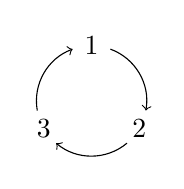
\begin{tikzpicture}[->,scale=.7]
               \node (1) at (90:1cm)  {$1$};
               \node (2) at (-30:1cm) {$2$};
               \node (3) at (210:1cm) {$3$};
            
               \draw (70:1cm)  arc (70:-10:1cm);
               \draw (-50:1cm) arc (-50:-130:1cm);
               \draw (190:1cm) arc (190:110:1cm);
            \end{tikzpicture}
            (Note $(1\;2\;3) = (2\;3\;1) = (3\;1\;2)$)
        \end{enumerate}
    \end{enumerate}
\end{example}


\begin{definition}
    Let $k_1,k_2,..., k_r \in \{1,2,...,n\}$ be distinct $(r \leq n)$. Then the permutation in $S_n$ which sends $k_1\mapsto k_2\mapsto k_3\mapsto ... \mapsto k_r \mapsto k_1$ and fixes all other numbers is denoted \begin{equation}
        (k_1\;k_2\;...\;k_r)
    \end{equation}
    which is a \Emph{cycle of length $r$} or an \Emph{$r$-cycle}.
\end{definition}

\begin{remark}
    The only $1$-cycle is the identity permutation in $S_n$
    \begin{enumerate}
        \item[$\rightarrow$] $(1) = (2) = ... = (n)$
    \end{enumerate}
\end{remark}

\begin{definition}
    Cycles of length $\geq 2$ in $S_n$ are called \Emph{disjoint} if they \emph{move} disjoint sets of numbers
    \begin{enumerate}
        \item[$\rightarrow$] \begin{example}
            $(1\;2), (3\;4)$ are disjoint in $S_4$, but $(1\;2),(3\;1)$ are \underline{not}.
        \end{example} 
    \end{enumerate}
\end{definition}


\begin{remark}
    Every permutation in $S_n$($\neq \id$), can be written as a product of disjoint cycles of length $\geq 2$. Moreover, this factorization is unique up to the order of the factors.
    \begin{proof}
        (Left to the reader)
    \end{proof}
\end{remark}

\begin{example}
    In $S_5$ $(1\;4\;5)\circ(2\;3) = (2\;3) \circ(1\;4\;5)$ as they are disjoint
    \begin{enumerate}
        \item[$\rightarrow$] (so we can't hope for full unicity of the factorization) 
    \end{enumerate}
\end{example}


\section{ General Properties}

\begin{definition}
    For a group $(G, \star)$, the number of elements (cardinal) of $G$ is denoted $|G|$ and called the \Emph{order} of the group (can be infinite).
\end{definition}

\begin{example}
    \begin{enumerate}
        \item $(\Z,+)$ has infinite order
        \item $(S_n,\circ)$ has order $n!$ (permutations)
    \end{enumerate}
\end{example}

\begin{proposition}
    Let $(G,\star)$ be a group. Then we have the following properties:
    \begin{enumerate}
        \item The identity element is unique.
        \begin{proof}
            If $e,i \in G$ are identity elements, then $e = e\star i = i$ as $e \star g = e$ and $g \star i = g$ for all $g \in G$ by assumption.
        \end{proof}
        \item The inverse of an element is unique.
        \begin{lemma}[Cancellation Lemma]
            If $a \star b = a \star c$ or $b \star = c \star a$, then $b = c$ for all $a,b,c \in G$. 
        \end{lemma}
        \begin{proof}
            Let $a^{-1}$ be an inverse of $a$. Then $$b = e\star b = (a^{-1} \star a) \star b = a^{-1} \star a \star c = e \star c = c$$ and similarly for $b \star a = c \star a$.
        \end{proof}
        \begin{remark}
            $a \star b = c \star a$ does \underline{not} tell us anything in general.
        \end{remark}
        \begin{proof}
            Take $b,c,$ inverses of $a$. Then $b \star a = e = c \star a$, so by the cancellation lemma $b = c$.
        \end{proof}
        \begin{enumerate}
            \item[$\rightarrow$] We will denote \underline{the} inverse of $a$ by $a^{-1}$ for all $a \in G$. 
        \end{enumerate}
        \begin{corollary}
            For all $a \in G$, if $b \star a = e$ (or $a \star b = e$) the identity element, then we have that $b = a^{-1}$, so $b$ is the inverse of $a$.
        \end{corollary}
    \end{enumerate}
\end{proposition}


\begin{definition}
    Let $(G, \star)$ be a group. Let $n \in \Z$, $g \in G$, then \begin{equation}
        g^n = \left\{\begin{array}{ll} e, & \text{if } n = 0 \\ \underbrace{g\star g \star ... \star g}_{\text{n-fold times}}, & \text{if } n > 0 \\ \underbrace{g^{-1}\star g^{-1} \star ... \star g^{-1}}_{\text{-n-fold times}}, & \text{if } n < 0\end{array}\right.
    \end{equation}
\end{definition}

\begin{proposition}
    For all $g \in G$ and all $n,m \in \Z$, \begin{enumerate}
        \item $(g^n)^m = g^{nm}$
        \item $g^n\star g^m = g^{n+m}$
    \end{enumerate}
    \begin{proof}
        (Left to the reader)
    \end{proof}
\end{proposition}

\begin{example}
    Let $G = \Z/2\Z$, $g = [1]$, and the operation be $+$. Then $g^{-1} = -1\cdot g = [-1] = [1]$, $g^0 = 0\cdot g = [0]$, $g^1 = 1\cdot g = [1]$, $g^2 = 2\cdot g = [1]+[1] = [2] = [0]$, and $g^3 = 3\cdot g = [3] = [1]$, etc.
\end{example}

\begin{remark}
    Due to associativity, the placement of parenthesis is unambiguous and unnecessary:
    $$\rightarrow ((a\star (b\star c)) \star d) = ((a \star b) \star (c \star d))$$
    Thus, $g_1\star g_2 \star ... \star g_n$ is well-defined for all $n \in \N$. 
    \begin{proof}
        (Left to the reader)
    \end{proof}
\end{remark}

\begin{note}
    However, because we don't necessarily have commutivity, it is \underline{not} true in general that $(g\star h)^n = g^n \star h^n$. Indeed, $(g\star h )^2 = g\star h \star g \star h$, not necessarily $g^2\star h^2$.
\end{note}

\begin{remark}[Inverse of a product]
    Let $a,b \in G$, a group. Then \begin{enumerate}
        \item $(a \star b)^{-1} = b^{-1}\star a^{-1}$
        \item More generally \begin{equation}
            (a_1\star a_2 \star ... \star a_n)^{-1} = a_n^{-1}\star ... \star a_2^{-1} \star a_1^{-1}
        \end{equation}
        for $a_i \in G$, $1 \leq i \leq n$
    \end{enumerate}
    \begin{proof}
        (Left to the reader)
    \end{proof}
\end{remark}

\begin{example}
    In $(\Z,+)$, $g^2$ for $g = 3$ is $g^2 = 2\cdot g = 2\cdot 3 = 6$. In general $g^n = ng$ for additive groups.
\end{example}

%
\section*{Appendix: Semi-Groups and Monoids}
%
\addcontentsline{toc}{section}{Appendix: Semi-Groups and Monoids}
    \begin{definition}
        A \Emph{semi-group} is a set $A$ equipped with a binary operation \begin{equation}
            A\times A \xrightarrow{mult} A,\;\;\;(a_1,a_2)\mapsto a_1\cdot a_2
        \end{equation}
        which satisfies the associativity axiom:\begin{equation}
            \forall a_1,a_2,a_3 \in A,\;\;\;a_1\cdot (a_2\cdot a_3) = (a_1\cdot a_2)\cdot a_3
        \end{equation}
        We can write this associativity axiom as the following commuting diagram:
        \begin{center}
            \begin{tikzpicture}[baseline = (a).base]
            \node[scale = 1] (a) at (0,0){
                \begin{tikzcd}
                    A\times A \times A \ar[d, "mult \times \id_A", swap] \ar[r, "\id_A\times mult"] & A\times A \ar[d,"mult"] \\
                    A\times A \ar[r, "mult"] & A
                \end{tikzcd}
            };
            \end{tikzpicture}
        \end{center}
    \end{definition}
    
    \begin{definition}
        A semi-group is said to be a \Emph{monoid} if there exists an element $1 \in A$ that satisfies \begin{equation}
            \forall a \in A,\;\;\;1\cdot a = a = a \cdot 1
        \end{equation}
        An element $1 \in A$ is called the \Emph{unity} or \Emph{identity} in $A$.
    \end{definition}
    
    \begin{lemma}
        A monoid contains a unique identity element.
        \begin{proof}
            (Left to the reader)
        \end{proof}
    \end{lemma}
    
    \begin{definition}
        An inverse of $a \in A$, a monoid, is an element $a^{-1} \in A$ such that \begin{equation}
            a\cdot a^{-1} = 1 = a^{-1} \cdot a
        \end{equation}
    \end{definition}
    
    \begin{lemma}
        If $a \in A$ admits an inverse, then this inverse is unique.
        \begin{proof}
            (Left to the reader)
        \end{proof}
    \end{lemma}
    
    \begin{definition}
        A monoid is said to be a \Emph{group} if every element admits an inverse.
    \end{definition}
    
    \begin{example}
        \leavevmode
        \begin{enumerate}
            \item $(\Z,+)$ is a group
            \item $(\Z,\cdot)$ is a monoid but not a group
            \item $(\R,+)$ is a group
            \item $(\R,\cdot)$ is a monoid but not a group ($0$ doesn't have an inverse)
            \item $(\R-\{0\},\cdot)$ is a group
            \item $\{\pm 1\} \subset \R$ with the operation $\cdot$ is a group.
            \item $(\C-\{0\},\cdot)$ is a group
            \item $(\{z\in \C-\{0\}:|z| = 1\},\cdot$ is a group, often denoted $S^1$ (the \Emph{circle group})
        \end{enumerate}
    \end{example}
    
    \begin{definition}
        A semi-group/monoid/group $A$ is said to be \Emph{commutative} if \begin{equation}
            \forall a_1,a_2 \in A,\;\;\;a_1\cdot a_2 = a_2\cdot a_1
        \end{equation}
        We call such a structure \Emph{abelian}. We may rewrite the commutativity condition as the commutative diagram:
        \begin{center}
            \begin{tikzpicture}[baseline = (a).base]
            \node[scale = 1] (a) at (0,0){
                \begin{tikzcd}
                    A\times A  \ar[d, "swap_A", swap] \ar[r, "mult"] & A \ar[d,"\id_A"] \\
                    A\times A \ar[r, "mult"] & A
                \end{tikzcd}
            };
            \end{tikzpicture}
        \end{center}
        where for any set $X$, $\map{swap_X:X\times X\rightarrow X\times X}{(x_1,x_2)\mapsto (x_2,x_1)}$
    \end{definition}
